

\tikzset{every picture/.style={line width=0.75pt}} %set default line width to 0.75pt        

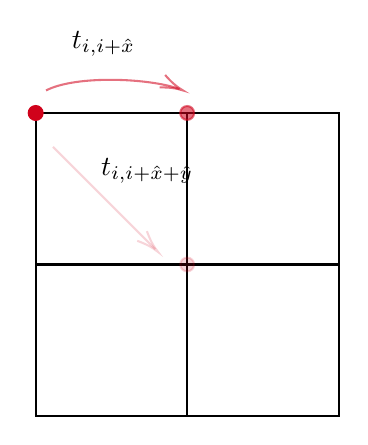
\begin{tikzpicture}[x=0.75pt,y=0.75pt,yscale=-1,xscale=1]
%uncomment if require: \path (0,300); %set diagram left start at 0, and has height of 300

%Shape: Grid [id:dp9196204391144727] 
\draw  [draw opacity=0] (186,104) -- (332,104) -- (332,250) -- (186,250) -- cycle ; \draw   (259,104) -- (259,250) ; \draw   (186,177) -- (332,177) ; \draw   (186,104) -- (332,104) -- (332,250) -- (186,250) -- cycle ;
%Straight Lines [id:da29204160455087] 
\draw [color={rgb, 255:red, 208; green, 2; blue, 27 }  ,draw opacity=0.56 ][fill={rgb, 255:red, 208; green, 2; blue, 27 }  ,fill opacity=0.13 ]   (259,104) ;
\draw [shift={(259,104)}, rotate = 0] [color={rgb, 255:red, 208; green, 2; blue, 27 }  ,draw opacity=0.56 ][fill={rgb, 255:red, 208; green, 2; blue, 27 }  ,fill opacity=0.56 ][line width=0.75]      (0, 0) circle [x radius= 3.35, y radius= 3.35]   ;
%Straight Lines [id:da29894868694295185] 
\draw [color={rgb, 255:red, 208; green, 2; blue, 27 }  ,draw opacity=0.17 ]   (194.33,120.33) -- (243.59,169.59) ;
\draw [shift={(245,171)}, rotate = 225] [color={rgb, 255:red, 208; green, 2; blue, 27 }  ,draw opacity=0.17 ][line width=0.75]    (10.93,-3.29) .. controls (6.95,-1.4) and (3.31,-0.3) .. (0,0) .. controls (3.31,0.3) and (6.95,1.4) .. (10.93,3.29)   ;
%Straight Lines [id:da865515748256444] 
\draw [color={rgb, 255:red, 208; green, 2; blue, 27 }  ,draw opacity=1 ][fill={rgb, 255:red, 208; green, 2; blue, 27 }  ,fill opacity=1 ]   (186,104) ;
\draw [shift={(186,104)}, rotate = 0] [color={rgb, 255:red, 208; green, 2; blue, 27 }  ,draw opacity=1 ][fill={rgb, 255:red, 208; green, 2; blue, 27 }  ,fill opacity=1 ][line width=0.75]      (0, 0) circle [x radius= 3.35, y radius= 3.35]   ;
%Straight Lines [id:da24429470745271376] 
\draw [color={rgb, 255:red, 208; green, 2; blue, 27 }  ,draw opacity=0.17 ][fill={rgb, 255:red, 208; green, 2; blue, 27 }  ,fill opacity=1 ]   (259,177) ;
\draw [shift={(259,177)}, rotate = 0] [color={rgb, 255:red, 208; green, 2; blue, 27 }  ,draw opacity=0.17 ][fill={rgb, 255:red, 208; green, 2; blue, 27 }  ,fill opacity=0.17 ][line width=0.75]      (0, 0) circle [x radius= 3.35, y radius= 3.35]   ;
%Curve Lines [id:da1801641720051903] 
\draw [color={rgb, 255:red, 208; green, 2; blue, 27 }  ,draw opacity=0.56 ]   (191,93.15) .. controls (205.4,85.65) and (241,87.19) .. (255.32,92.47) ;
\draw [shift={(257,93.15)}, rotate = 204.12] [color={rgb, 255:red, 208; green, 2; blue, 27 }  ,draw opacity=0.56 ][line width=0.75]    (10.93,-3.29) .. controls (6.95,-1.4) and (3.31,-0.3) .. (0,0) .. controls (3.31,0.3) and (6.95,1.4) .. (10.93,3.29)   ;

% Text Node
\draw (202,63.4) node [anchor=north west][inner sep=0.75pt]    {$t_{i,i+\hat{x}}$};
% Text Node
\draw (216,124.4) node [anchor=north west][inner sep=0.75pt]    {$t_{i,i+\hat{x} +\hat{y}}$};


\end{tikzpicture}
